\entry{Semana del 28/04/2025}

\section{Miércoles 30/04/2025}

\subsection*{Resumen Rápido}

\begin{itemize}
	\item Estaba lista la impresión del conector entre el tornillo y el perfil. Las dimensiones estaban bien pero la ficha T es muy grande, queda poco espacio por encima y no encastra bien el perfil.
	\item Estaban las piezas de ELEMON.
	\item Pablo consiguió el alambre de cobre de 0.35 mm de diámetro.
	\item También de ELEMON un esmalte aislante "aislamatic".
\end{itemize}

Empecé a probar el funcionamiento del circuito RLC y la parte conceptual del funcionamiento del sensor. No fue posible conectar el osciloscopio Siglent a la computadora, sí el generador Tektronix. 

Básicamente armé en la protoboard un circuito RLC con R=1.8 k$\Omega$ (aunque la cinta decía que era de 1 k$\Omega$), H = 10 mH y C=100 pF. Luego, con la resistencia conectada en una punta a Tierra levanté con el osciloscopio la caída de potencial sobre la misma (para que no haga corto con la Tierra del generador) y ajusté la frecuencia de resonancia (para que ambas señales estuvieran en fase), que había dado ligeramente distinta a la esperada teóricamente. 

\begin{figure}[!ht]
	\centering
	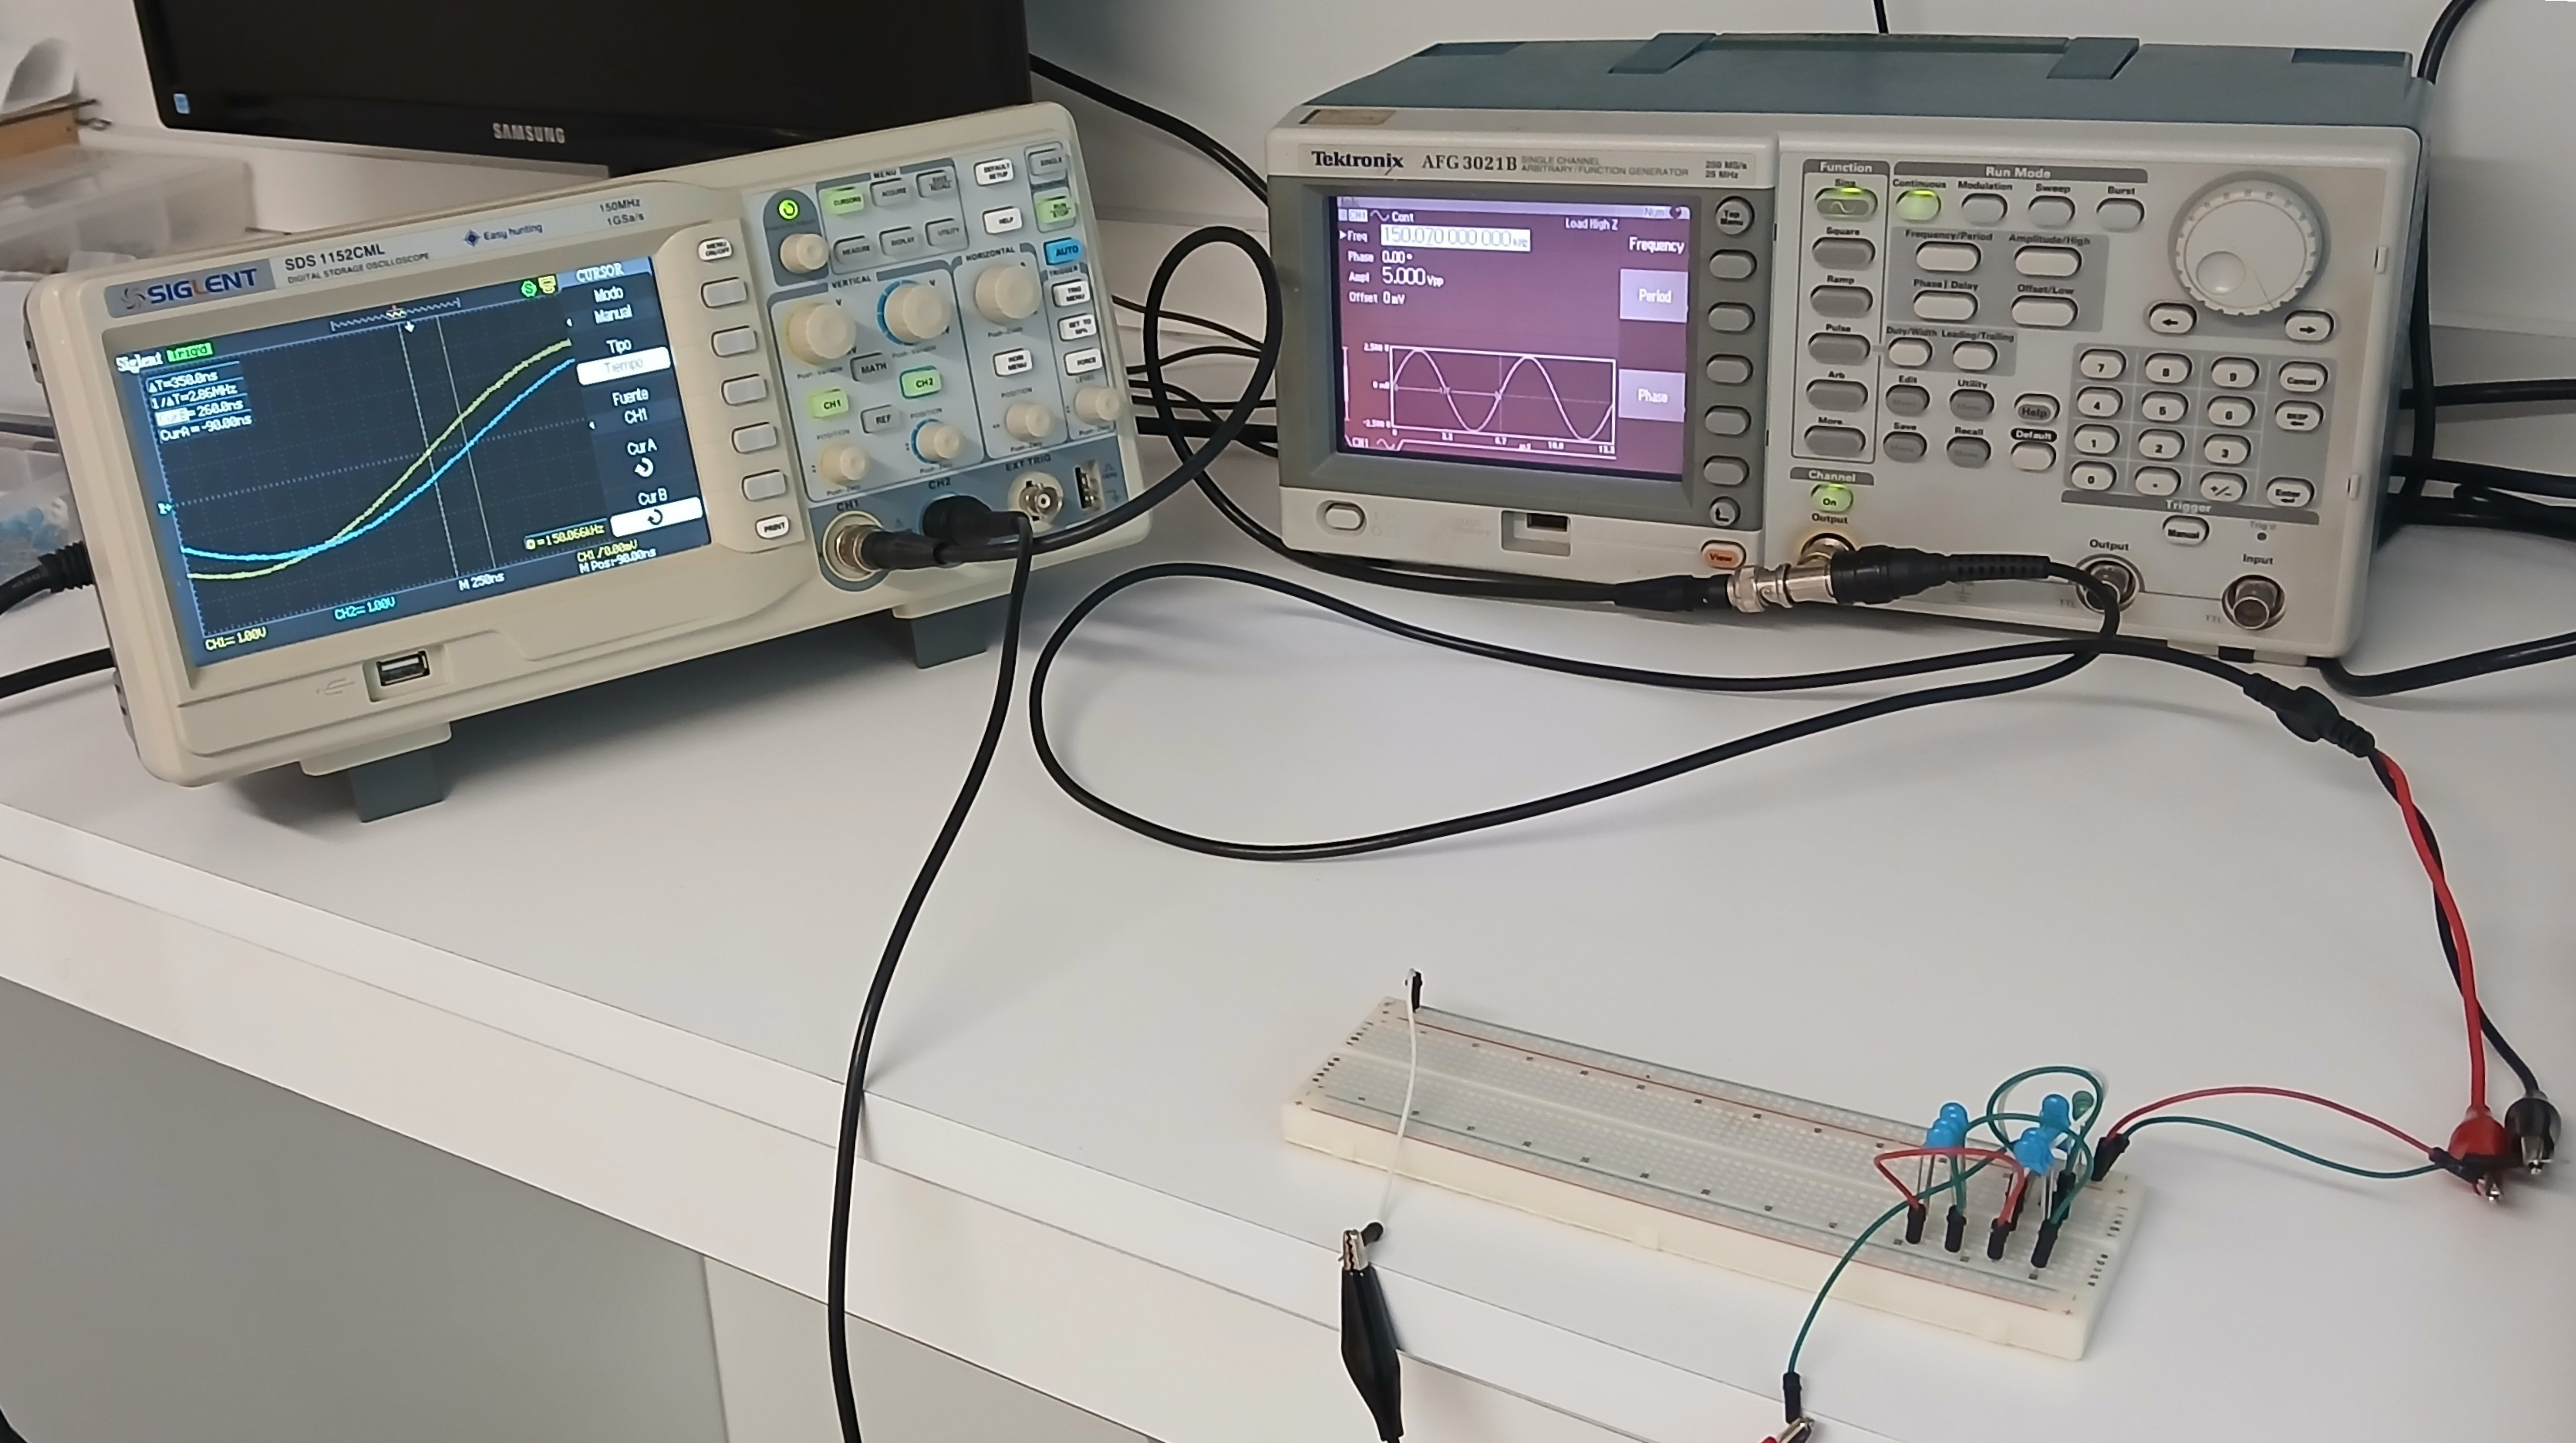
\includegraphics[width=0.675\linewidth]{Figures/28_04_2025/20250430_162448.JPG}
	
	\vspace{5.01mm}
	
	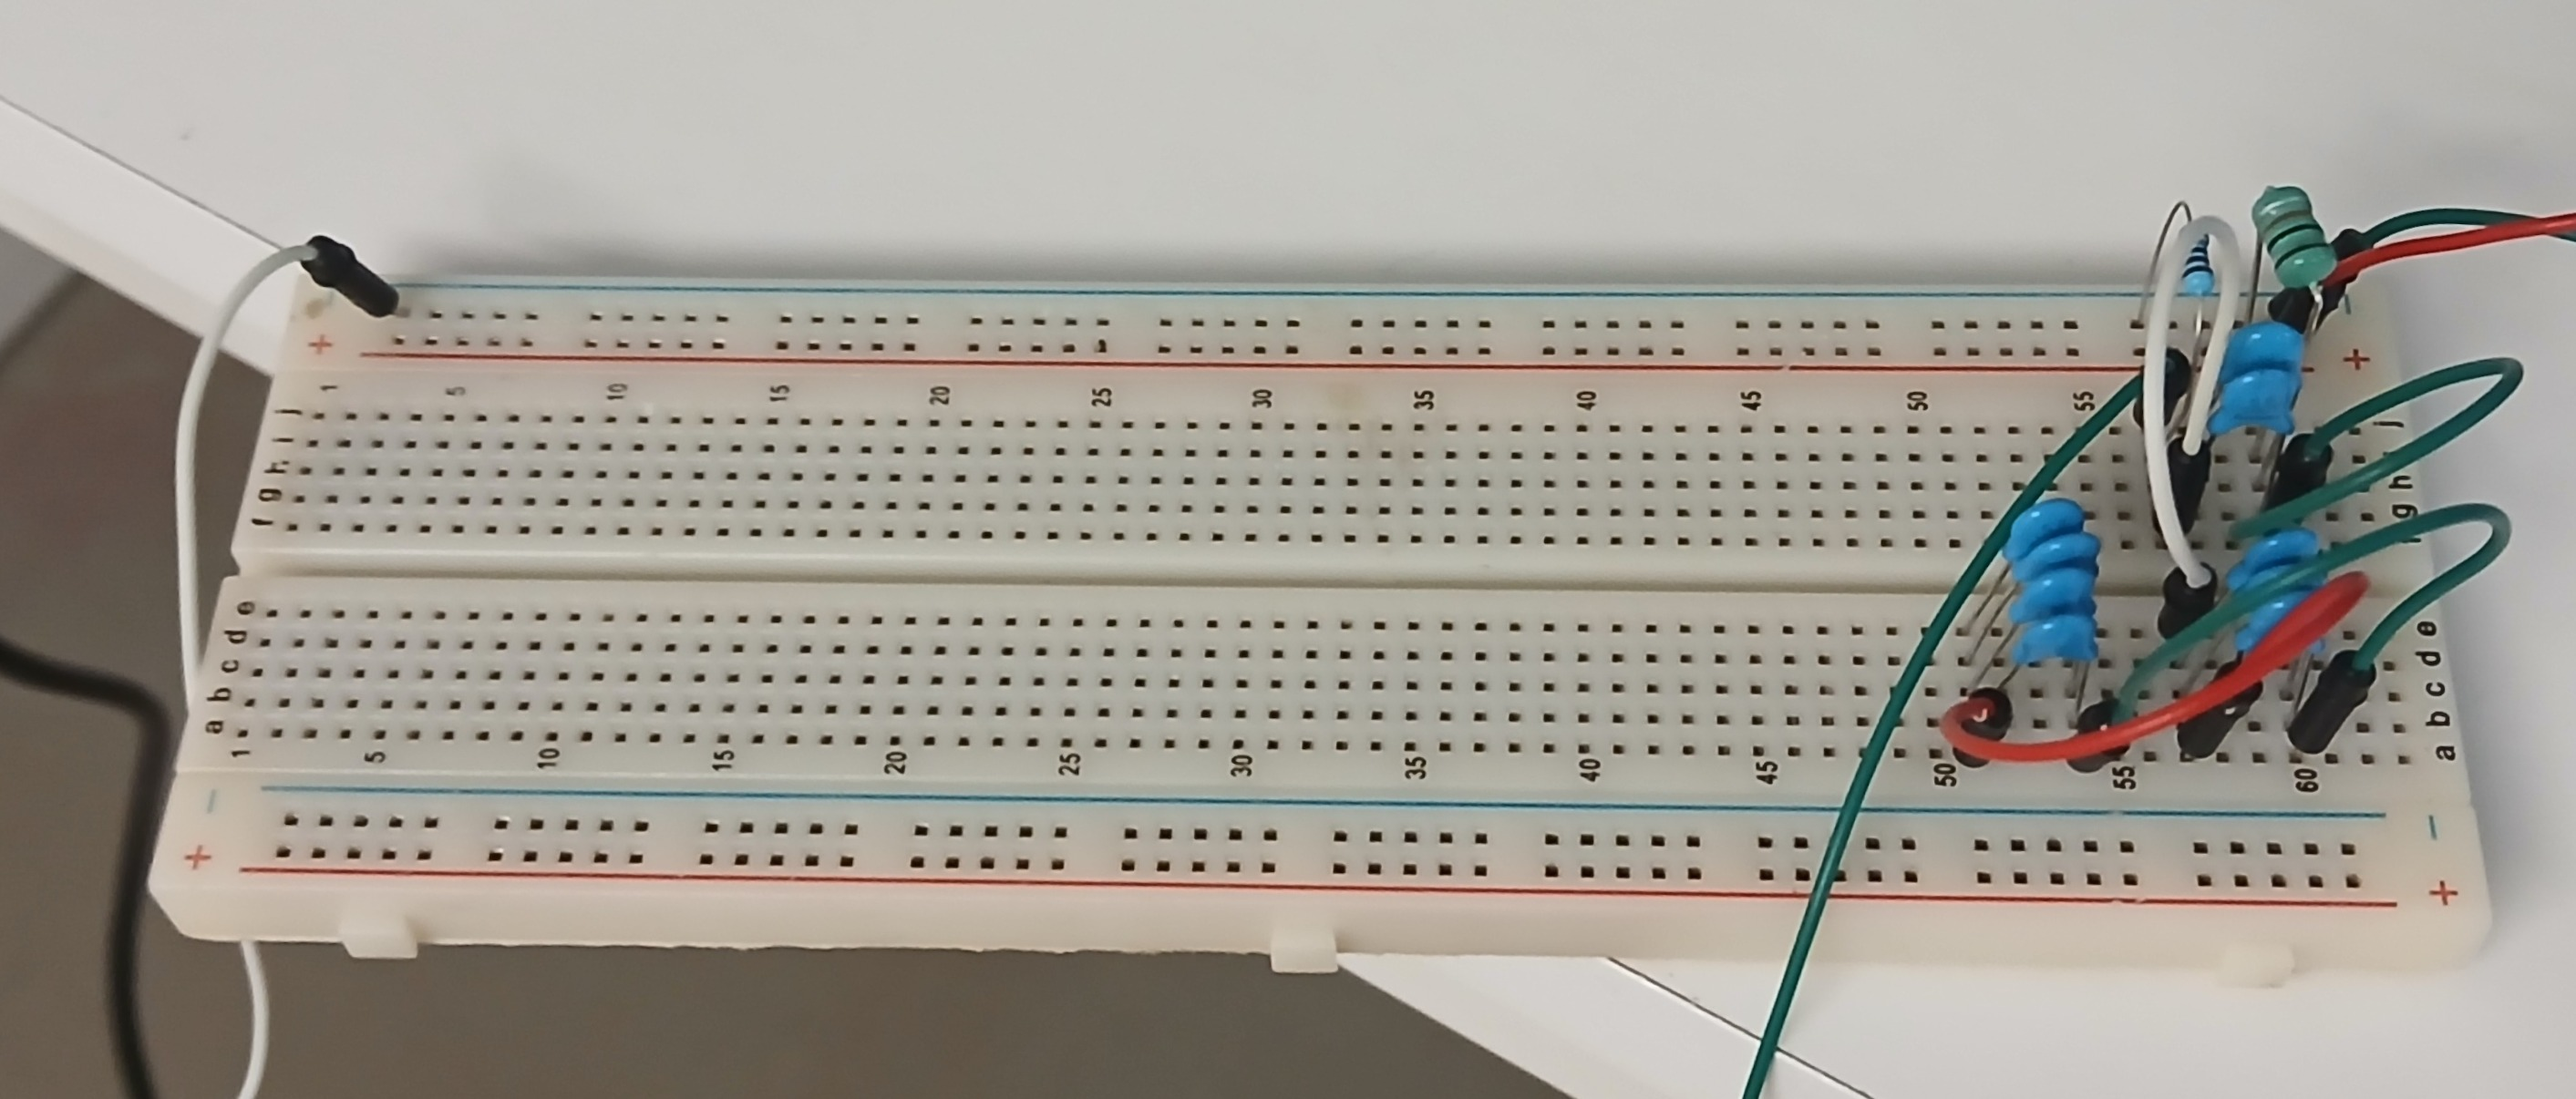
\includegraphics[width=0.675\linewidth]{Figures/28_04_2025/20250430_160622.JPG}
	\caption{Arriba foto general del setup para el RLC con el osciloscopio y el generador de funciones. Abajo la forma de poner capacitancias en paralelo a la principal $C_0$.}
	\label{fig:fotos_28_05_2025}
\end{figure}

Después empecé a poner en paralelo a la capacitancia más grande otras de un par de órdenes de magnitud más chica, para ver si efectivamente esto cambiaba linealmente la fase. Como no pude conectar el oscilosocpio a la computadora para calcular la fase lo hice calculando el $\Delta T$ entre los dos cursores de la pantalla, cada uno puesto en el 0 de ambas señales (la de referencia de generador de funciones y la caída de voltaje sobre la resistencia). Luego si se quisiera se puede convertir a fase multiplicando por la frecuencia 

\begin{equation}
	\phi = \omega \Delta T % r 
\end{equation}	

Abajo están los resultados de esta primera prueba. Al agregar las capacitancias de 5.6 pF se nota que se comporta más o menos lineal hasta unos 15 pF total agregados y después satura como cuando resolvíamos numéricamente la ecuación diferencial del RLC con $C=C(t)$.


\begin{figure}[!ht]
	\centering
	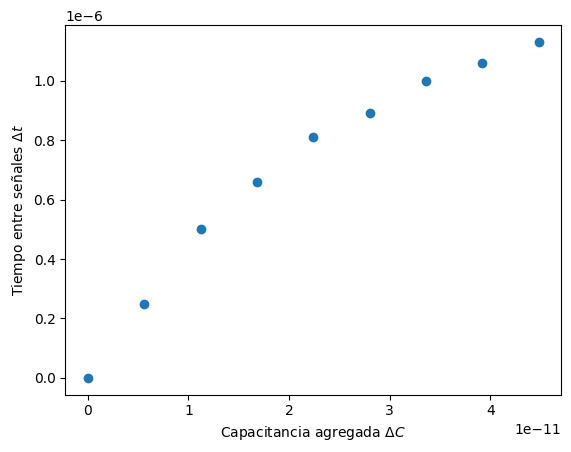
\includegraphics[width=0.6157\linewidth]{Figures/28_04_2025/Barrido_grande}
	\caption{Agregado de capacitancias de 5.6 pF en paralelo a la de 100 pF para ver cómo variaba la fase del circuito.}
	\label{fig:barridogrande}
\end{figure}

Después haciendo un barrido mucho más fino se observa que efectivamente el comportamiento para capacitancias chicas es lineal: % a 

\begin{figure}[!ht]
	\centering
	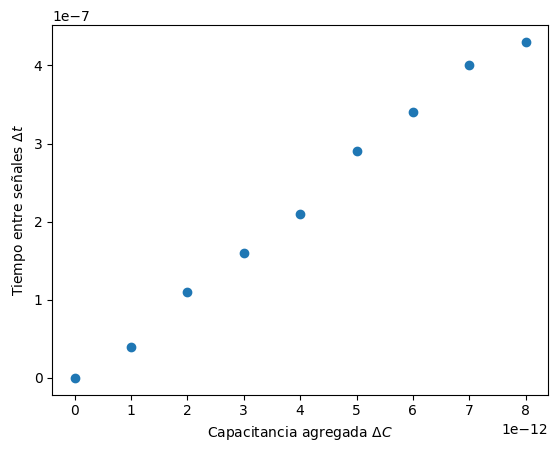
\includegraphics[width=0.6157\linewidth]{Figures/28_04_2025/Barrido_chico}
	\caption{Agregado de capacitacnias de 1 pF en paralelo a la de 100 pF.}
	\label{fig:barridochico}
\end{figure}

Con lo cual si de verdad para el sensor $C=C'\Delta l $ y $C\ll C_0$ entonces podríamos usarlo como queremos. Ya que $\Delta l$ sería proporcional a $\phi$ con alguna constante de proporcionalidad que encontraríamos calibrando el sensor, al desplazarlo una distancia conocida $\Delta l$ en el agua y midiendo el $\phi$ resultante de esta operación. 

